\documentclass[11pt]{amsart}
\usepackage[a4paper,margin=1in]{geometry}
\usepackage{amsmath,amssymb,amsthm}
\usepackage{tikz}
\usepackage[hidelinks]{hyperref}

\newtheorem{thm}{Theorem}
\newtheorem{lemma}{Lemma}
\theoremstyle{definition}
\newtheorem{example}{Example}
\newtheorem{remark}[thm]{Remark}

\title[Hankel determinants of path generating functions]{Cigler's Hankel determinants of path generating functions do not depend on the horizontal weight}
\author{Vamshi Jandhyala}
\address{London, United Kingdom}
\date{Preprint, version 1, 18 November 2026. Not peer reviewed.}
\subjclass[2020]{05A15, 15A15, 05A19}
\keywords{Hankel determinant, Motzkin path, lattice path, ballot numbers, Catalan-like numbers}

\begin{document}

\begin{abstract}
Weight the horizontal steps of a Motzkin path by $c+x$ at height $0$ and by $c$ above it, and let $a_{n,k}$ count the
paths of length $n$ from height $0$ to height $k$. Cigler observed that the Hankel determinants
$\det(a_{i+j,k})_{0\le i,j<n}$ seem not to depend on $c$, and that they appear to equal the determinant of a
band matrix $H_{k,n}(x)$ of ones and powers of $x$. The first statement follows from the classical invariance of Hankel
determinants under binomial transforms. We prove the second for all $k$ and $n$: cutting each path in two turns the
Hankel determinant into a determinant of path counts between heights, and that path-count matrix factors as $H_{k,n}(x)$
times a unitriangular matrix of ballot numbers.
The proof is formalised in Lean. Cigler's further quadratic recurrence for these determinants remains open.
\end{abstract}

\maketitle

\section{Introduction}

Motzkin paths are walks that move one unit to the right at each step and go up, down or straight across, never
dropping below the horizontal axis. Weighting their steps and counting them gives the moments of orthogonal
polynomials, and Hankel determinants of such counts are a classical source of identities. Cigler asked about one
weighting~\cite{MO,C23}. Up and down steps have weight $1$. A horizontal step has weight $c+x$ at height $0$
and weight $c$ at every height above. The weighted count $a_{n,k}=a_{n,k}(x,c)$ of paths from $(0,0)$ to $(n,k)$ obeys
\[
a_{n,k}=a_{n-1,k-1}+s_k\,a_{n-1,k}+a_{n-1,k+1},\qquad s_0=c+x,\quad s_l=c\ (l\ge1),
\]
with $a_{0,k}=[k=0]$ and $a_{n,-1}=0$. Cigler studied
\[
D_{k,n}(x,c)=\det\big(a_{i+j,k}(x,c)\big)_{0\le i,j\le n-1}.
\]

\begin{example}\label{ex:small}
Take $k=1$ and $n=3$. The entries are $a_{0,1}=0$, $a_{1,1}=1$, $a_{2,1}=2c+x$, $a_{3,1}=3c^2+3cx+x^2+2$ and
$a_{4,1}=4c^3+6c^2x+4cx^2+8c+x^3+3x$, so
\[
D_{1,3}=\det\begin{pmatrix}0&1&2c+x\\ 1&2c+x&3c^2+3cx+x^2+2\\ 2c+x&3c^2+3cx+x^2+2&a_{4,1}\end{pmatrix}=x.
\]
Several entries depend on $c$, and all of that dependence cancels.
\end{example}

Cigler computed many such values and conjectured that $c$ never matters~\cite[p.~5]{C23}; he had asked the same question about shifting the horizontal weights in 2022~\cite{MSE}. He also proposed an
explicit replacement. Let $H_{k,n}(x)=(h_{i,j})_{0\le i,j\le n-1}$ with $h_{k-m+l,\,m+l}=1$ for $0\le m\le k$ and
$l\ge0$, with $h_{l,\,k+i+l}=x^i$ for $i\ge1$ and $l\ge0$, and with all other entries $0$. For example
\[
H_{2,6}(x)=\begin{pmatrix}
0&0&1&x&x^2&x^3\\ 0&1&0&1&x&x^2\\ 1&0&1&0&1&x\\ 0&1&0&1&0&1\\ 0&0&1&0&1&0\\ 0&0&0&1&0&1
\end{pmatrix}.
\]
The ones lie on the $k+1$ diagonals where the column index minus the row index is one of $-k,-k+2,\dots,k$, starting
from the antidiagonal through $(0,k)$; the powers of $x$ fill the corner above them.

\begin{thm}\label{thm:main}
For all $k\ge0$ and $n\ge0$, the determinant $D_{k,n}(x,c)$ does not depend on $c$, and
\[
D_{k,n}(x,c)=\det H_{k,n}(x).
\]
\end{thm}

The first statement is not new. Adding $c$ to every horizontal weight replaces the sequence $m\mapsto a_{m,k}$ by its
transform $\sum_j\binom mj c^{\,m-j}a_{j,k}$, and Hankel determinants are invariant under this transform: Layman proved
it for $c=1$~\cite{L01}, and Spivey and Steil for every $c$ (their falling $c$-binomial transform)~\cite[Theorem~6.1]{SS06}; Petrov gives the same unitriangular argument in a MathOverflow answer~\cite{P22}.
The short proof is in Section~\ref{sec:step1}. The content of
Theorem~\ref{thm:main} is the second statement. For $x=0$ it was known that $D_{k,n}$ takes only the values $0$ and
$\pm1$~\cite[p.~5]{C23}, and Chern and Shi~\cite{CS} evaluate the related determinants when the boundary weight is $b=0$
or $b=1$ in Cigler's notation, which is our $x$. We found no earlier proof of the identity with $\det H_{k,n}(x)$ for
general $x$.

\emph{The route.} The classical step comes first: a binomial transform multiplies a Hankel matrix by a unitriangular
matrix on each side, so $c$ drops out (Section~\ref{sec:step1}). With $c=0$, cut each path of length $i+j$ after $i$ steps (Figure~\ref{fig:cut}).
The first piece runs from height $0$ to some height $l\le i$, and the matrix of those counts is again unitriangular, so
the Hankel determinant equals a determinant of path counts from height $l$ to height $k$ in $j$ steps
(Section~\ref{sec:step2}). Finally that matrix factors as $H_{k,n}(x)$ times a matrix of ballot numbers, which is
unitriangular and depends on neither $k$ nor $x$ (Section~\ref{sec:step3}). The whole of the content sits in one local
identity for the entries of $H$, equation~\eqref{eq:local}.

\section{Removing \texorpdfstring{$c$}{c}}\label{sec:step1}

This section is classical~\cite{L01,SS06}; we give the argument in the form used below.
Each horizontal step carries weight $c$, plus an extra $x$ at height $0$. Expand the product of weights along a path
of length $n$: choosing the summand $c$ at some set of horizontal steps and deleting those steps leaves a path of
length $j$ with weights $(x,0,0,\dots)$, and the deleted steps can sit in any $n-j$ of the $n$ positions. Hence
\begin{equation}\label{eq:binom}
a_{n,k}(x,c)=\sum_{j=0}^{n}\binom nj c^{\,n-j}\,a_{j,k}(x,0).
\end{equation}
The left side is a path count with the constant $c$ present; the right side builds it from paths without $c$, by
choosing where the $c$-steps go. By Vandermonde's identity,
$\binom{i+j}{t}c^{\,i+j-t}=\sum_{r+s=t}\binom ir c^{\,i-r}\binom js c^{\,j-s}$, so \eqref{eq:binom} gives
\[
\big(a_{i+j,k}(x,c)\big)_{i,j}=L\,\big(a_{i+j,k}(x,0)\big)_{i,j}\,L^{T},\qquad L=\Big(\binom ir c^{\,i-r}\Big)_{i,r},
\]
with $L$ lower unitriangular. Taking determinants of the leading $n\times n$ blocks, $D_{k,n}(x,c)=D_{k,n}(x,0)$.

The argument never used the special shape of the weights: adding one constant to all horizontal weights leaves every
determinant $\det(a_{i+j,k})_{0\le i,j<n}$ unchanged, for any weight sequence $s_0,s_1,\dots$. From now on $c=0$, so
horizontal steps occur only at height $0$, with weight $x$.

\section{Cutting the paths}\label{sec:step2}

Write $W_j(l\to k)$ for the weighted number of paths of length $j$ from height $l$ to height $k$ that never go below
$0$, with the weights of Section~\ref{sec:step1} at $c=0$. Thus $a_{j,k}=W_j(0\to k)$.

\begin{figure}[ht]
\centering
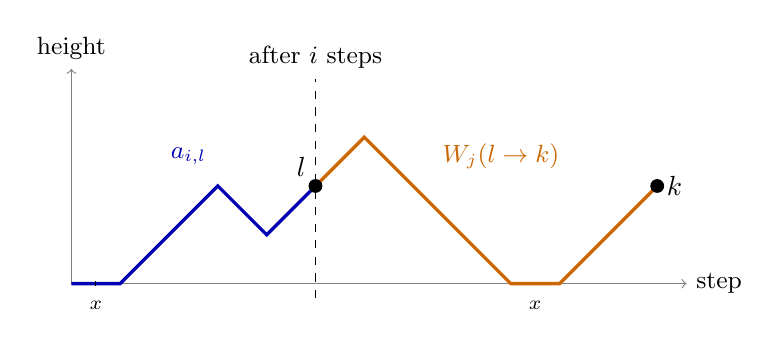
\begin{tikzpicture}[x=0.62cm,y=0.62cm]
  \draw[->,gray] (0,0) -- (12.6,0) node[right,black] {\small step};
  \draw[->,gray] (0,0) -- (0,4.4) node[above,black] {\small height};
  \draw[dashed] (5,-0.3) -- (5,4.2) node[above] {\small after $i$ steps};
  \draw[very thick,blue!70!black] (0,0) -- (1,0) -- (2,1) -- (3,2) -- (4,1) -- (5,2);
  \draw[very thick,orange!80!black] (5,2) -- (6,3) -- (7,2) -- (8,1) -- (9,0) -- (10,0) -- (11,1) -- (12,2);
  \fill (5,2) circle (2.5pt) node[above left] {$l$};
  \fill (12,2) circle (2.5pt) node[right] {$k$};
  \node[blue!70!black] at (2.4,2.6) {\small $a_{i,l}$};
  \node[orange!80!black] at (8.8,2.6) {\small $W_j(l\to k)$};
  \draw (0.5,-0.05) -- (0.5,0.05);
  \node[font=\scriptsize] at (0.5,-0.45) {$x$};
  \node[font=\scriptsize] at (9.5,-0.45) {$x$};
\end{tikzpicture}
\caption{A path of length $i+j=12$ from height $0$ to height $k=2$, cut after $i=5$ steps. The first piece is counted
by $a_{i,l}$ and the second by $W_j(l\to k)$; horizontal steps (weight $x$) occur only on the floor.}
\label{fig:cut}
\end{figure}

\begin{lemma}\label{lem:cut}
$D_{k,n}=\det\big(W_j(l\to k)\big)_{0\le l,j\le n-1}$.
\end{lemma}

\begin{proof}
Cutting a path of length $i+j$ after $i$ steps (Figure~\ref{fig:cut}) gives
\[
a_{i+j,k}=\sum_{l=0}^{i}a_{i,l}\,W_j(l\to k).
\]
The matrix $(a_{i,l})_{0\le i,l\le n-1}$ is lower unitriangular: a path of length $i$ cannot reach a height above $i$,
and reaches height $i$ in exactly one way, by going up every time. So the Hankel matrix is this unitriangular matrix
times $\big(W_j(l\to k)\big)_{l,j}$, and the determinants agree.
\end{proof}

\section{The factorisation}\label{sec:step3}

Extend $H$ to an infinite matrix with rows $l\ge0$ and columns $s\ge0$; its leading $n\times n$ block is $H_{k,n}(x)$.
Unpacking the definition,
\begin{equation}\label{eq:H}
H_{l,s}=\begin{cases}x^{\,s-l-k}, & s-l>k,\\ 1, & |s-l|\le k,\ l+s\ge k,\ l+s\equiv k \pmod 2,\\ 0,&\text{otherwise.}\end{cases}
\end{equation}
In words: above the band the entry records how far the column outruns the row, as a power of $x$; inside the band
there is a one wherever the parity is right and the antidiagonal $l+s=k$ has been reached.

Let $B(j,i)$ be the ballot numbers, the number of paths of $j$ up and down steps from height $0$ to height $i$ that
never go below $0$. They satisfy $B(0,i)=[i=0]$ and $B(j,i)=B(j-1,i-1)+B(j-1,i+1)$, with $B(j,-1)=0$, and
$B(j,i)=0$ for $i>j$. Put $U=\big(B(j,i)\big)_{i,j}$, with row $i$ and column $j$; it is upper unitriangular, and it
depends on neither $k$ nor $x$.

\begin{lemma}\label{lem:factor}
For all $l,j\ge0$,
\begin{equation}\label{eq:factor}
W_j(l\to k)=\sum_{i=0}^{j}H_{l,i}\,B(j,i).
\end{equation}
\end{lemma}

The left side counts weighted paths from height $l$ to height $k$; the right side reads row $l$ of $H$ against the
ballot paths of length $j$. The proof is an induction on $j$, and its one real ingredient is a local identity for $H$:
with the conventions $H_{l,-1}=H_{-1,i}=0$,
\begin{equation}\label{eq:local}
H_{l,i+1}+H_{l,i-1}=H_{l-1,i}+H_{l+1,i}+x\,[l=0]\,H_{0,i}\qquad(l,i\ge0).
\end{equation}
Read left to right, it says that moving one column right or left along row $l$ of $H$ adds up to the same as moving one
row up or down along column $i$, with a correction $x\,H_{0,i}$ on the floor. That is the shape of the path recursion:
the ballot recursion acts on the columns of $H$ and the step recursion for $W$ acts on its rows.

\begin{proof}[Proof of \eqref{eq:local}]
Two facts follow directly from \eqref{eq:H}. Shifting $l$ and $s$ together keeps $s-l$ and the parity of $l+s$ and
changes only the condition $l+s\ge k$; and row $0$ is $H_{0,s}=x^{\,s-k}[s\ge k]$. Hence
\[
H_{l+1,i+1}=H_{l,i}+[l+i+2=k],\qquad H_{0,i+1}=x\,H_{0,i}+[i+1=k]\qquad(l\ge0,\ i\ge-1).
\]
For $l\ge1$, apply the first fact at $(l-1,i)$ and at $(l,i-1)$: $H_{l,i+1}=H_{l-1,i}+[l+i+1=k]$ and
$H_{l+1,i}=H_{l,i-1}+[l+i+1=k]$. Subtracting gives \eqref{eq:local}. For $l=0$, the first fact at $(0,i-1)$ gives
$H_{1,i}=H_{0,i-1}+[i+1=k]$; adding the second fact gives \eqref{eq:local}.
\end{proof}

\begin{proof}[Proof of Lemma~\ref{lem:factor}]
For $j=0$, \eqref{eq:factor} says $H_{l,0}=[l=k]$, which is \eqref{eq:H} at $s=0$. Suppose \eqref{eq:factor} holds for
$j-1$. The ballot recursion and then \eqref{eq:local} give
\[
\sum_i H_{l,i}B(j,i)=\sum_i B(j-1,i)\big(H_{l,i+1}+H_{l,i-1}\big)
=\sum_iB(j-1,i)\big(H_{l-1,i}+H_{l+1,i}+x[l=0]H_{0,i}\big).
\]
By the induction hypothesis the right side is $W_{j-1}(l-1\to k)+W_{j-1}(l+1\to k)+x[l=0]\,W_{j-1}(0\to k)$, with
$W_{j-1}(-1\to k)=0$. Splitting off the first step of a path from height $l$, this is $W_j(l\to k)$.
\end{proof}

\begin{proof}[Proof of Theorem~\ref{thm:main}]
Since $B(j,i)=0$ for $i>j$, restricting \eqref{eq:factor} to $0\le l,j\le n-1$ gives
$\big(W_j(l\to k)\big)_{l,j}=H_{k,n}(x)\,U_n$, where $U_n$ is the leading block of $U$ and has determinant $1$.
With Lemma~\ref{lem:cut} and Section~\ref{sec:step1},
$D_{k,n}(x,c)=D_{k,n}(x,0)=\det H_{k,n}(x)$.
\end{proof}

\section{Remarks}\label{sec:remarks}

\emph{What the factorisation shows.} The ballot matrix $U$ is the same for every $k$ and every $x$. All the dependence
on the target height and the boundary weight sits in $H$: its band of ones carries the contributions with no
horizontal step (such walks may still touch the floor), and its powers of $x$ count the horizontal steps taken on it.

\emph{The open recurrence.} Cigler also observed that for $n\ge2k+2$,
\[
d_{k,n}\,d_{k,n-2k-2}-x^2\,d_{k,n-1}\,d_{k,n-2k-1}=(1-x^2)\,d_{k,n-k-1}^2,\qquad d_{k,n}=\det H_{k,n}(x),
\]
see~\cite[equation~(18)]{C23}, where it is stated with $b$ in place of $x$. For $k=1$ it follows from Cassini's identity
for Fibonacci polynomials~\cite{C23}. We have checked it numerically for $k\le5$ and $n<22$ and have not proved it.
Theorem~\ref{thm:main} reduces it to a statement about the band matrices $H_{k,n}(x)$ alone.

\section{Verification}\label{sec:verify}

Theorem~\ref{thm:main} is formalised in Lean~4 with Mathlib, over an arbitrary commutative ring, so that $x$ and $c$ may
be indeterminates. The matrix $H_{k,n}(x)$ is written exactly as in Cigler's definition, and the case $k=0$ is
included. The formalisation also proves the general remark of Section~\ref{sec:step1} for every weight sequence, and
checks the displayed $H_{2,6}(x)$ and the value $D_{1,3}=x$ of Example~\ref{ex:small}. It uses only Lean's standard
axioms, and every planted wrong statement in a mutation suite is rejected. Separately, one program compares
$D_{k,n}(x,c)$ at two values of $c$ with $\det H_{k,n}(x)$ at random integer points for $1\le k\le5$ and $n<22$, and
checks the open recurrence in the same range; a second program, sharing no code with it, checks each step of the proof
symbolically (the binomial transform, the cutting identity and the factorisation~\eqref{eq:factor}) for small $k$, $n$. The scripts and the
Lean project are in the folder \texttt{cigler-hankel-paths} of \url{https://github.com/jvvk/mathematics} and, identical
to that folder at tag \texttt{cigler-hankel-paths-v1}, in the Zenodo record \href{https://doi.org/10.5281/zenodo.24353081}{doi:10.5281/zenodo.24353081}.

\section*{Declaration of generative AI and AI-assisted technologies in the research and writing process}
During the preparation of this work the author used Claude (Anthropic; model Claude Opus~5.5) to find the proof, write
the verification code and the Lean formalisation, and draft the text, and Codex (OpenAI) to review the release
independently. The author directed the work and takes full responsibility for the content of the publication. This
first version is released before the author's own line-by-line reading of the text; the proof is formalised in Lean, as
described in Section~\ref{sec:verify}.

\begin{thebibliography}{9}

\bibitem{CS} S.~Chern and W.~Shi, Hankel determinants of Catalan-like sequences, arXiv:2608.27208v1 (2026).

\bibitem{C23} J.~Cigler, Some results and conjectures about Hankel determinants of sequences which are related to
Catalan-like numbers, arXiv:2309.15557v1 (2023).

\bibitem{L01} J.~W.~Layman, The Hankel transform and some of its properties, \emph{J.\ Integer Seq.} \textbf{4} (2001),
Article 01.1.5.

\bibitem{MSE} J.~Cigler, Hankel determinants related to Motzkin paths, Mathematics Stack Exchange question 4428971
(16 April 2022), \url{https://math.stackexchange.com/q/4428971}, accessed 18 November 2026.

\bibitem{MO} J.~Cigler, A conjecture about Hankel determinants of path generating functions, MathOverflow question
456683 (2023), \url{https://mathoverflow.net/q/456683}, accessed 18 November 2026.

\bibitem{P22} F.~Petrov, answer to ``A coincidence or a fact: determinants of two matrices'', MathOverflow answer 428093
(8 August 2022), \url{https://mathoverflow.net/a/428093}, accessed 18 November 2026.

\bibitem{SS06} M.~Z.~Spivey and L.~L.~Steil, The $k$-binomial transforms and the Hankel transform, \emph{J.\ Integer
Seq.} \textbf{9} (2006), Article 06.1.1.

\end{thebibliography}
\end{document}
